\begin{figure}[H]
  \centering
  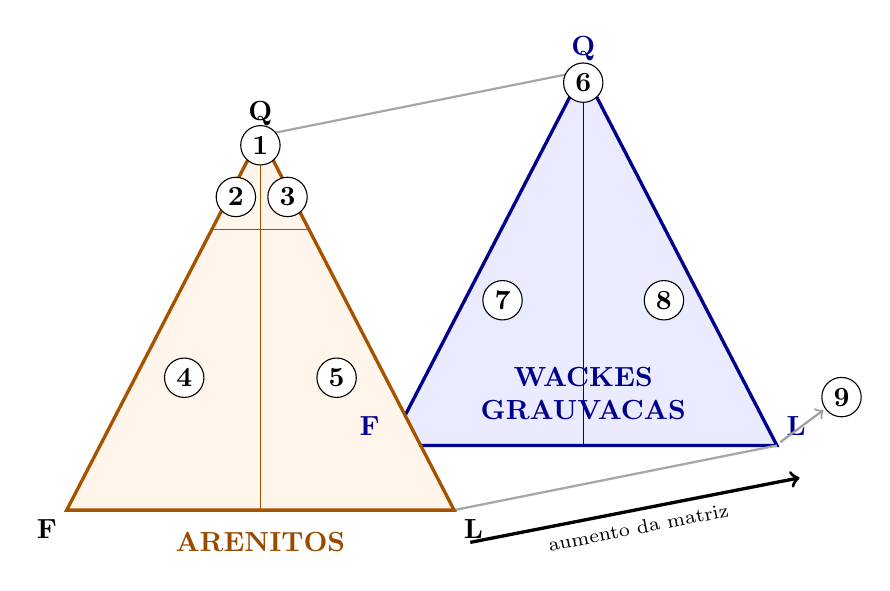
\begin{tikzpicture}[x=0.82cm,y=0.82cm,font=\scriptsize]
    % Triângulo posterior: wackes
    \coordinate (Qb) at (5,6.8);
    \coordinate (Fb) at (2,1.0);
    \coordinate (Lb) at (8,1.0);
    \path[fill=blue!8] (Qb)--(Fb)--(Lb)--cycle;
    \draw[very thick,blue!55!black] (Qb)--(Fb)--(Lb)--cycle;
    \draw[blue!55!black] (Qb)--(5,1.0);
    \draw[blue!55!black] (4.85,6.51)--(5.15,6.51);

    % Arestas que formam o prisma triangular
    \draw[gray!70,thick] (0,5.8)--(Qb);
    \draw[gray!70,thick] (-3,0)--(Fb);
    \draw[gray!70,thick] (3,0)--(Lb);

    % Triângulo anterior: arenitos/arenitas
    \coordinate (Q) at (0,5.8);
    \coordinate (F) at (-3,0);
    \coordinate (L) at (3,0);
    \path[fill=orange!8] (Q)--(F)--(L)--cycle;
    \draw[very thick,orange!65!black] (Q)--(F)--(L)--cycle;
    \draw[orange!65!black] (-0.15,5.51)--(0.15,5.51); % Q = 95%
    \draw[orange!65!black] (-0.75,4.35)--(0.75,4.35); % Q = 75%
    \draw[orange!65!black] (Q)--(0,0);                % F = L

    % Polos composicionais
    \node[above,font=\bfseries] at (Q) {Q};
    \node[below left,font=\bfseries] at (F) {F};
    \node[below right,font=\bfseries] at (L) {L};
    \node[above,font=\bfseries,text=blue!55!black] at (Qb) {Q};
    \node[above left,font=\bfseries,text=blue!55!black] at (Fb) {F};
    \node[above right,font=\bfseries,text=blue!55!black] at (Lb) {L};

    % Numeração dos campos; a nomenclatura aparece na lista abaixo.
    \tikzset{campo/.style={circle,draw,fill=white,inner sep=1.2pt,
      minimum size=5mm,font=\bfseries}}

    % Arenitas
    \node[campo] at (0,5.65) {1};
    \node[campo] at (-0.38,4.85) {2};
    \node[campo] at (0.42,4.85) {3};
    \node[campo] at (-1.18,2.05) {4};
    \node[campo] at (1.18,2.05) {5};
    \node[font=\bfseries,orange!60!black] at (0,-0.5)
      {ARENITOS};

    % Wackes
    \node[campo] at (5,6.62) {6};
    \node[campo] at (3.75,3.25) {7};
    \node[campo] at (6.25,3.25) {8};
    \node[
        font=\bfseries,
        blue!55!black,
        align=center
    ] at (5,1.8)
        {WACKES\\GRAUVACAS};

    % Terceira dimensão do esquema
    \draw[->,very thick] (3.25,-0.50)--(8.35,0.50)
      node[midway,below,sloped] {aumento da matriz};
    \node[campo] at (9.0,1.75) {9};
    \draw[->,gray!75,thick] (8.05,1.05)--(8.72,1.55);
  \end{tikzpicture}

  \vspace{0.5em}
  \begin{tabularx}{0.98\linewidth}{@{}rX rX@{}}
    \toprule
    \multicolumn{4}{c}{\textbf{Nomenclatura dos campos}} \\
    \midrule
    1. & Quartzoarenito
       & 6. & Wacke quartzosa \\
    2. & Subarcóseo
       & 7. & Wacke feldspática \\
    3. & Sublitoarenito
       & 8. & Wacke lítica \\
    4. & Arcóseo / arenito feldspático
       & 9. & Pelito: matriz acima de 75\% \\
    5. & Litoarenito / arenito lítico
       & & \\
    \bottomrule
  \end{tabularx}
  \caption{Classificação prismática dos arenitos pelo teor de matriz e pela
  composição Q--F--L do arcabouço: Q = quartzo, F = feldspatos e
  L = fragmentos líticos.}
  \label{fig:classificacao-arenitos-prisma}
  \caption*{\footnotesize Fonte: adaptado da classificação de Pettijohn apresentada
  por \textcite{nichols2009}.}
\end{figure}
